% =====================================================================
% main-uis.tex — Versión con formato UIS (Universidad Industrial de
% Santander): portada, agradecimientos, tabla de contenido, lista de
% figuras, lista de tablas, lista de apéndices, resumen y abstract.
% Genera main-uis.pdf con las figuras a resolución completa, sin tocar
% el build de trabajo (main.tex / main.pdf).
% Compilar: latexmk -lualatex main-uis.tex
% =====================================================================
\documentclass[12pt, a4paper, oneside]{book}
\usepackage{iftex}

% ======================
% Language
% ======================
\ifPDFTeX
  \usepackage[T1]{fontenc}
  \usepackage[utf8]{inputenc}
  \usepackage{lmodern}
  \usepackage{textalpha}
  \usepackage{textgreek}
  \providecommand{\greekfont}{}
\else
  \usepackage{fontspec}
  \setmainfont{Latin Modern Roman}
  \setsansfont{Latin Modern Sans}
  \setmonofont{Latin Modern Mono}
  \newfontfamily{\greekfont}[Script=Greek]{GFS Didot}
\fi
\usepackage[spanish,es-tabla,es-nodecimaldot]{babel}
% babel-spanish redefine \% para insertar un espacio fino automático; en modo
% matemático eso choca con el \, explícito ("Incompatible glue units").
\spanishplainpercent
\usepackage{csquotes}

% Nombres de las secciones preliminares según el formato UIS
\addto\captionsspanish{%
  \renewcommand{\contentsname}{Tabla de contenido}%
  \renewcommand{\listfigurename}{Lista de figuras}%
  \renewcommand{\listtablename}{Lista de tablas}%
}

% ======================
% Page Layout (encabezado UIS: título corrido en cursiva mayúscula a la
% izquierda, folio a la derecha, filete horizontal)
% ======================
\usepackage[a4paper, margin=2.5cm]{geometry}
\usepackage{fancyhdr}
\setlength{\headheight}{15pt}

\fancypagestyle{uis}{%
  \fancyhf{}%
  \fancyhead[L]{\itshape\MakeUppercase{\leftmark}}%
  \fancyhead[R]{\thepage}%
  \renewcommand{\headrulewidth}{0.4pt}%
  \renewcommand{\footrulewidth}{0pt}%
}
% Folio inferior centrado, sin encabezado (páginas de Resumen y Abstract)
\fancypagestyle{uisfolioinferior}{%
  \fancyhf{}%
  \fancyfoot[C]{\thepage}%
  \renewcommand{\headrulewidth}{0pt}%
  \renewcommand{\footrulewidth}{0pt}%
}
% Las primeras páginas de capítulo usan el mismo encabezado UIS
\fancypagestyle{plain}{%
  \fancyhf{}%
  \fancyhead[L]{\itshape\MakeUppercase{\leftmark}}%
  \fancyhead[R]{\thepage}%
  \renewcommand{\headrulewidth}{0.4pt}%
  \renewcommand{\footrulewidth}{0pt}%
}
\pagestyle{uis}

% En clase oneside el mark de capítulo va a \markright; lo llevamos a
% \markboth para que \leftmark siempre contenga el título corrido.
\renewcommand{\chaptermark}[1]{%
  \markboth{\ifnum\value{chapter}>0 \thechapter.\ \fi #1}{}}

% ======================
% Hyperlinks & TOC
% ======================
\usepackage[hidelinks]{hyperref}
\hypersetup{unicode=true}
\setcounter{secnumdepth}{3}
\setcounter{tocdepth}{3}
\usepackage{enumitem}

% Listas de figuras y tablas con la palabra completa (formato UIS)
\usepackage[titles]{tocloft}
\renewcommand{\cftfigpresnum}{Figura\ }
\renewcommand{\cftfigaftersnum}{.}
\setlength{\cftfignumwidth}{6.5em}
\renewcommand{\cfttabpresnum}{Tabla\ }
\renewcommand{\cfttabaftersnum}{.}
\setlength{\cfttabnumwidth}{6em}

% ======================
% Mathematics
% ======================
\usepackage{amsmath, amssymb, mathtools, bm}
\usepackage{mathrsfs}   % for \mathscr
\usepackage{physics}
\usepackage{cancel}

\usepackage{lettrine}
\usepackage{algorithm}
\usepackage[noend]{algpseudocode}
\floatname{algorithm}{Algoritmo}
\renewcommand{\algorithmicrequire}{\textbf{Entrada:}}
\renewcommand{\algorithmicensure}{\textbf{Salida:}}
\algrenewcommand{\algorithmicfor}{\textbf{para}}
\algrenewcommand{\algorithmicdo}{\textbf{hacer}}
\algrenewcommand{\algorithmicend}{\textbf{fin}}
\algrenewcommand{\algorithmicif}{\textbf{si}}
\algrenewcommand{\algorithmicthen}{\textbf{entonces}}
\algrenewcommand{\algorithmicelse}{\textbf{si no}}
\algrenewcommand{\algorithmicwhile}{\textbf{mientras}}
\algrenewcommand{\algorithmicreturn}{\textbf{retornar}}

% Numeración de ecuaciones por capítulo
\numberwithin{equation}{chapter}

% ======================
% Graphics
% ======================
\usepackage{graphicx}
\usepackage{tikz}
\usetikzlibrary{babel}
\usetikzlibrary{calc,angles,quotes,shapes.geometric}
\usepackage{pgfplots}
\pgfplotsset{compat=1.18}
\usepackage{float}
\usepackage{longtable}

% Este build usa siempre las figuras a resolución completa.
\newif\iffastbuild
\fastbuildfalse

% #1: graphicx options; #2: final asset; #3: optimized preview.
\newcommand{\thesisincludegraphics}[3][]{%
  \iffastbuild
    \includegraphics[#1]{#3}%
  \else
    \IfFileExists{#2}{%
      \includegraphics[#1]{#2}%
    }{%
      \PackageWarning{thesis}{Full-quality figure '#2' not found; using preview '#3'}%
      \includegraphics[#1]{#3}%
    }%
  \fi
}

% ======================
% Bibliography
% ======================
\usepackage[backend=biber,style=numeric,sorting=none]{biblatex}
\addbibresource{bibliography.bib}

% Commands
\newcommand{\uvec}[1]{\bm{\hat{\mathbf{#1}}}}
\newcommand{\mcal}[1]{\mathcal{#1}}
\newcommand{\lvec}[1]{\overrightarrow{#1}}

% Entrada de la lista de apéndices
\newcommand{\aplinea}[2]{%
  \par\noindent\hangindent=2.4em\hangafter=1
  #1~\dotfill~\pageref{#2}\par\addvspace{0.7em}}

% ======================
% Document
% ======================
\begin{document}

% ===== Portada (formato UIS) =====
\begin{center}
\noindent\rule{\textwidth}{0.4pt}\\[0.9em]
{\large Estudio de las aberraciones vectoriales en sistemas estigmáticos}\\[0.9em]
\rule{\textwidth}{0.4pt}

\vspace{3.2cm}
{\large Jhonatan S. Blanco}

\vspace{2.6cm}
{\large\itshape Trabajo de grado para optar al título de Físico}

\vspace{2.2cm}
{\large Director:}\\
{\large Rafael Ángel Torres Amarís}\\
{\large Físico, Mg., Dr.}

\vspace{1.1cm}
{\large Codirector:}\\
{\large Cristian Hernández Celis}\\
{\large Físico, Mg.}

\vfill
{\large Universidad Industrial de Santander}\\[0.2em]
{\large\scshape Facultad de ciencias}\\
{\large\scshape Escuela de física}\\
{\large\scshape Bucaramanga}\\
{\large 2026}
\end{center}
\clearpage

% ===== Agradecimientos =====
% ===== AGRADECIMIENTOS (solo main-uis.tex) =====
\chapter*{Agradecimientos}
\markboth{Agradecimientos}{Agradecimientos}

\lettrine[lines=2]{A}{gradecido} de forma inconmensurable con Dios, nuestro SEÑOR, por concebirme como criatura suya y hacerme parte de su magna creación. Maravillado estoy con la majestuosidad, elegancia, detalle, simplicidad, armonía, entre otras excelsas cualidades de la creación que Dios erigió como morada de sus criaturas y que parcialmente ha mostrado frente a mis ojos. Cada aspecto de la naturaleza el Señor con tanto cuidado lo pensó, y con la más infinita maestría lo ejecutó, y acá estamos ante el majestuoso sistema del mundo que el arquitecto universal erigió y por el cual su gloria es manifiesta, pues no hay lugar en la tierra o en las regiones supralunares donde tu gloria no sea manifiesta. Glorioso te muestras en la escala de las galaxias, dichoso te muestras en el átomo y tus procesos; todo lo dotaste de tanta vida, riqueza para comunicarse y cierto misterio que hace única cada cosa. Este mundo es magno, grande, lleno de gloria y obedece a tu palabra, que en el principio del mundo pronunciaste para que todo se crease y avanzara en armonía hacia tus propósitos. Nos lo entregaste a nosotros para su cuidado y como materia prima para nuestras creaciones, porque como creadores nos concebiste, pues nos hiciste a tu imagen y semejanza. Un mundo nos entregaste y un mundo te entregaremos, y DIOS, como agradecimiento por haberme creado y darme siempre salud y gran vitalidad en toda mi vida, me comprometo a hacer lo que en mí esté para pulir la tierra en la que habito. Y no solo mi compromiso es con la tierra que carece de tu aliento vital, sino también con tus hijos, pues en cuanto a mí esté, elevaré los espíritus de quienes hagan parte de mi camino hacia la verdad, lo bello y, en suma, lo que es correcto y bueno.

Gracias le doy a nuestro SEÑOR por mostrarme varios de los misterios de la naturaleza e iniciarme en ellos; gracias por hacerme parte de esta maravillosa creación, y aún más agradecido por no concebir el universo sin mi alma en él. Gracias por tenerme en tus propósitos, y gracias por mostrarme caminos dignos de seguir.

Agradezco a la humanidad por haber reconocido en la ciencia un instrumento para encontrar la verdad y mostrarle a todo el mundo la gloria de la creación; gracias por haberle puesto nombre y sistema a la filosofía de la naturaleza, gracias por la lengua que me enseñaron para comunicarme con mis contemporáneos y posiblemente con las generaciones venideras.

Quiero agradecer por darme una madre que siempre cuidó bien de mí, quiso lo mejor para mí y me apoyó mientras encontraba la manera de defenderme en este mundo y encontrar por mí mismo el sustento.

Gracias quiero dar al programa Generación E: Excelencia del Estado Colombiano, que me ayudó en mi sustento; sin dicho apoyo hubiese sido muy difícil haber concluido mis estudios. Por tanto, doy gracias y espero que siempre se apoye, y con el tiempo en mayor medida, el talento nacional y el buen encaminamiento de los jóvenes.

Esto es: gracias, Dios, por concebirme como hijo tuyo; gracias por darme una muy buena madre; gracias por darme el lenguaje y cierta inteligencia para entender algunos fenómenos de la naturaleza; gracias por el apoyo y las oportunidades, las que ya han pasado y todas las que vendrán.

\bigskip

\begin{center}
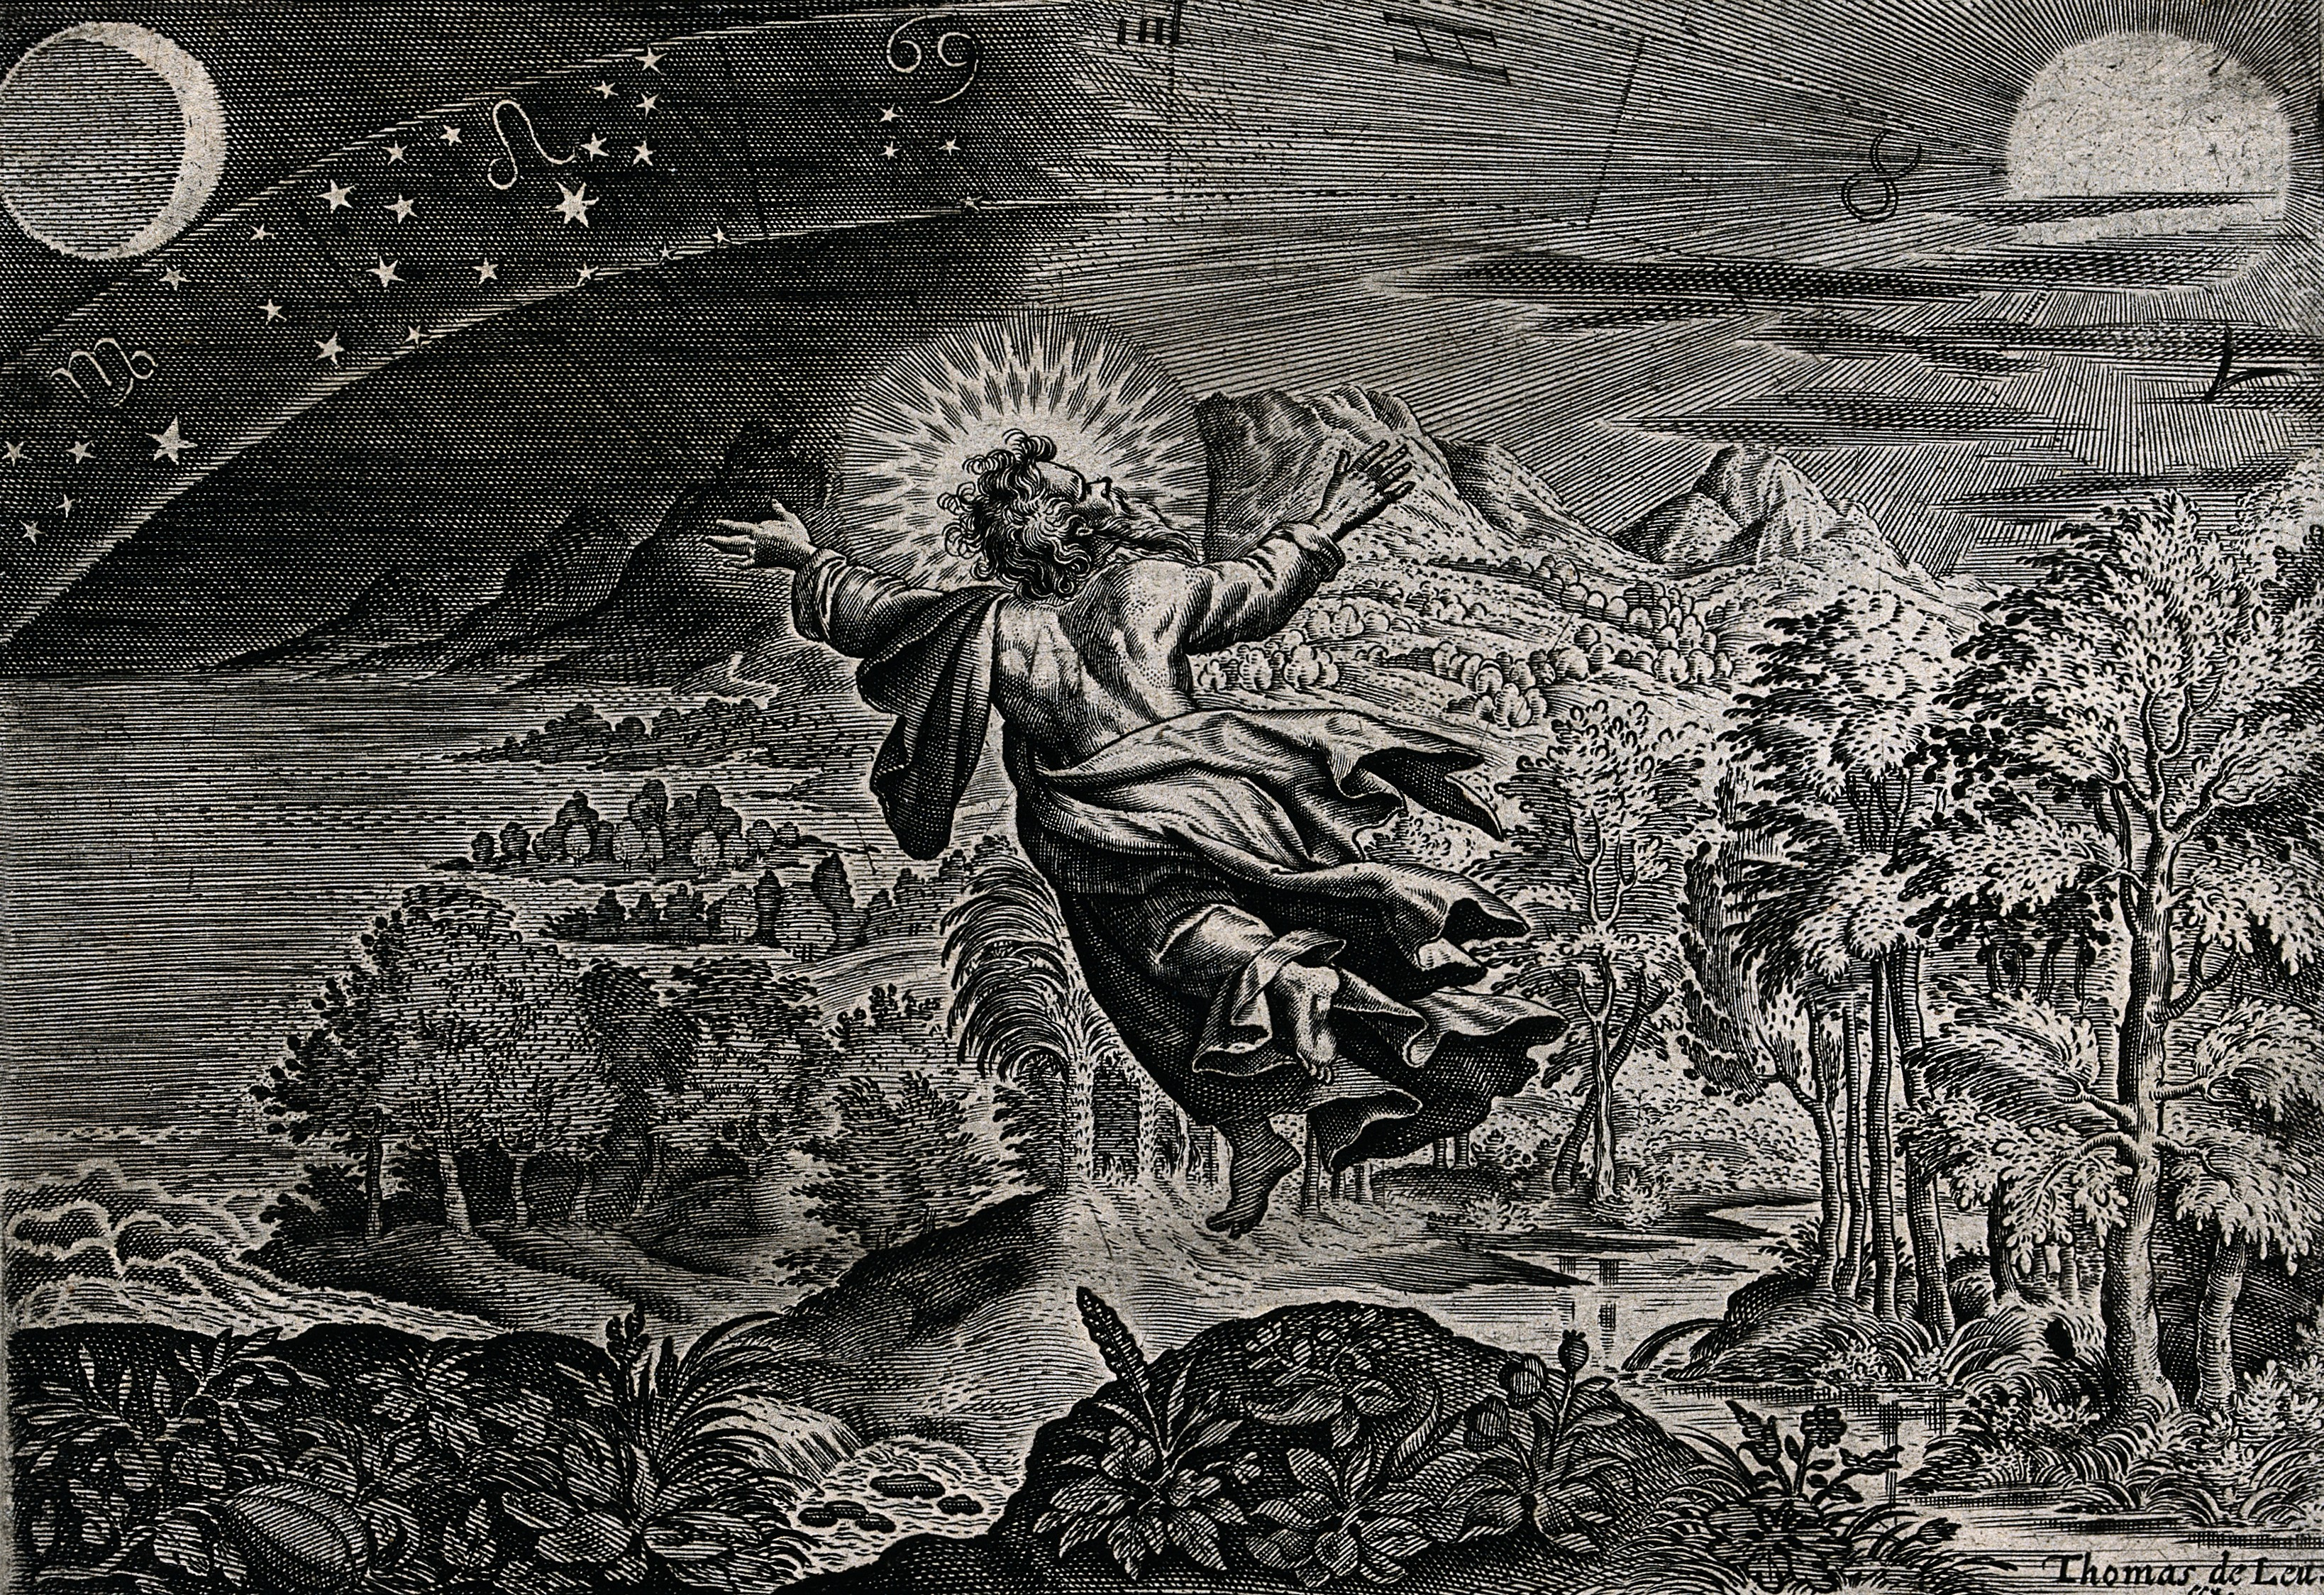
\includegraphics[width=0.7\textwidth]{figures/god_creates_sun_moon_stars.jpg}

{\small\itshape God creates the sun, moon and stars. Thomas de Leu. (1600).}

\vspace{0.7cm}
\textsc{Solo tú, Dios, eres la verdad, y a tu gloria consagro mi vida.}
\end{center}

\medskip

\begin{flushright}
\textsc{Tu humilde y sincero siervo,}\\[0.7em]
\textit{Jhonatan S. Blanco.}
\end{flushright}

\clearpage


% ===== Tabla de contenido =====
\tableofcontents
\clearpage

% ===== Lista de figuras =====
\listoffigures
\clearpage

% ===== Lista de tablas =====
\listoftables
\clearpage

% ===== Lista de apéndices =====
\chapter*{Lista de apéndices}
\markboth{Lista de apéndices}{Lista de apéndices}
\vspace{1em}
{\setlength{\parindent}{0pt}
\aplinea{Apéndice A.\enspace Transformada de Fourier bidimensional en coordenadas polares}{sec:fourier_2d_polar}
\aplinea{Apéndice B.\enspace Condiciones de frontera y coeficientes de Fresnel en dieléctricos}{sec:appendix_maxwell_frontera_fresnel}
\aplinea{Apéndice C.\enspace Deducción de la ecuación implícita del dioptrio estigmático}{apx:ovoid_implicit_deduction}
\aplinea{Apéndice D.\enspace Expansión en series para las superficies cartesianas y cantidades asociadas}{apx:ovoids_series}
\aplinea{Apéndice E.\enspace Pupila circular uniforme: resultados analíticos}{apx:focal_forms}
\aplinea{Apéndice F.\enspace Algoritmo de cálculo del campo focal}{apx:numerical_algorithm}
}
\clearpage

% ===== Resumen y Abstract (folio inferior, sin encabezado) =====
\fancypagestyle{plain}{%
  \fancyhf{}%
  \fancyfoot[C]{\thepage}%
  \renewcommand{\headrulewidth}{0pt}%
  \renewcommand{\footrulewidth}{0pt}%
}
\input{resumen.tex}
\clearpage
\fancypagestyle{plain}{%
  \fancyhf{}%
  \fancyhead[L]{\itshape\MakeUppercase{\leftmark}}%
  \fancyhead[R]{\thepage}%
  \renewcommand{\headrulewidth}{0.4pt}%
  \renewcommand{\footrulewidth}{0pt}%
}

% ======================

\input{chapters/00.Notacion_y_convenciones.tex}

\chapter*{Introducción}
\addcontentsline{toc}{chapter}{Introducción}
\markboth{Introducción}{Introducción}

\lettrine[lines=2]{L}{os} sistemas estigmáticos son de gran importancia en
la óptica, debido a que resuelven el problema de la formación de una imagen
perfecta de un objeto puntual en la óptica geométrica
\cite{bornwolf1999,Tyc2011Absolute}, con aplicaciones directas en la
microscopía de superresolución y la litografía óptica
\cite{Shen2022,flagello1996}, el procesamiento láser de materiales
\cite{Niziev1999Cutting} y el atrapamiento óptico de partículas
\cite{Kozawa2010Trapping}.

El estigmatismo es un importante punto de partida para el estudio
de la formación de imágenes \cite{singlet2020, bornwolf1999}. Las Superficies Cartesianas aseguran esta
condición en la refracción entre dos medios homogéneos y permiten construir
sistemas mediante su composición \cite{singlet2020,ovoids2023}. Una elección
adecuada de las Superficies Cartesianas permite obtener propiedades como el
aplanatismo y el acromatismo, lo que demuestra su utilidad y potencial en el
diseño óptico \cite{aplan2020,achro2022}.

La minimización de las aberraciones geométricas conserva su importancia aun
en la óptica física, donde estas se manifiestan como aberraciones de fase
que alteran el campo en la imagen \cite{bornwolf1999,goodman2005}. La relación directa con la función aberración de fase y la longitud de camino óptico, permite deducir que en los sistemas estigmaticos esta aberración es nula. Esta propiedad hace de las Superficies Cartesianas un
escenario apropiado para aislar las aberraciones vectoriales, pues permite
estudiar la transformación de amplitud y polarización sin mezclarla con
defectos de camino óptico. Aun así, la difracción produce una distribución
extendida,
descrita por la función de dispersión de punto (PSF, por sus siglas en inglés),
y establece limitaciones de resolución cuya referencia clásica es el límite
de Abbe \cite{Abbe1873,goodman2005}. La descripción escalar no permite
identificar los efectos de la polarización sobre esa distribución. Las
variaciones de amplitud y polarización sobre la pupila pueden deformar la
PSF y reducir el contraste de la imagen aun sin aberración de fase, lo que
motiva su estudio mediante una descripción vectorial
\cite{McGuire1991Response,mcguire1994,flagello1996}.

El impacto de estos efectos alcanza tanto la formación de imágenes como la
interacción de la luz con la materia. En litografía de alta apertura
numérica, la polarización modifica la distribución de intensidad y las
asimetrías de la imagen \cite{flagello1996}. En microscopía de
superresolución, las aberraciones de polarización pueden alterar el mínimo
de intensidad de los haces de agotamiento y los patrones de iluminación
estructurada. En microscopía polarimétrica, pueden introducir errores en
la información de polarización atribuida a la muestra \cite{Shen2022}.
Asimismo, la
polarización condiciona la eficiencia axial y transversal de las pinzas
ópticas \cite{Kozawa2010Trapping} y la absorción de energía que determina la
eficiencia del corte láser \cite{Niziev1999Cutting}. Estas aplicaciones
motivan la caracterización de las alteraciones de amplitud y polarización
introducidas por la refracción, incluso cuando la aberración de fase ya se
ha eliminado.

El tratamiento electromagnético dispone de representaciones integrales
exactas basadas en identidades vectoriales de Green \cite{StrattonChu1939}
y de métodos numéricos como el de elementos finitos (FEM) y el de diferencias
finitas en el dominio del tiempo (FDTD), cuyo costo computacional dificulta
el estudio de sistemas grandes respecto de la longitud de onda
\cite{Shi2019Curved,Wende2022,Song2025}. Las aproximaciones de Debye y
Richards--Wolf permiten un cálculo focal eficiente, pero presentan
restricciones de validez y, en el modelo aplanático ideal de
Richards--Wolf, omiten la transmisión diferencial de Fresnel en las
superficies de la lente
\cite{RichardsWolf1959,Sheppard2013Debye,Shi2019RealLenses,Wang2020Debye}.
Otros métodos incorporan la transmisión local mediante trazado vectorial,
aproximaciones de interfaz plana y operaciones espectrales
\cite{Kim18,Shi2019Curved,Wende2022,Song2025}.\footnote{El presente
desarrollo es independiente de los trabajos de Shi et
al.~\cite{Shi2019Curved} y Song et al.~\cite{Song2025}, conocidos durante
la revisión bibliográfica posterior.} Sin embargo, estos tratamientos
generales no caracterizan las aberraciones vectoriales de las Superficies
Cartesianas, y el antecedente específico de difracción vectorial en estas
superficies considera su apodización, pero excluye los coeficientes de
Fresnel en la comparación focal \cite{GonzalezAcuna2022Oval}. Queda así por
determinar la contribución de la transmisión vectorial a la estructura del
campo focal en ausencia de aberración de fase.

El objetivo de este trabajo es aislar y caracterizar las aberraciones de
origen netamente vectorial que estan presentes aun en ausencia de aberración de
fase. Para ello se calcula el campo eléctrico transmitido hacia el plano focal de una Superficie Cartesiana entre dos medios dieléctricos homogéneos e isótropos, donde el campo incidente es una onda esférica centrada en el punto objeto.
Este sistema es el sistema estigmático más simple, y nos permite examinar los efectos de la refracción vectorial sin la contribución de las aberraciones de camino óptico. 
En este trabajo expresamos la transmisión de forma operacional, dado el campo incidente mediante el operador matricial que se contruyó en este trabajo, damos el campo transmitido sobre la esféra gaussiana centrada en el punto imagen, matriz que a su vez, nos permite caracterizar la aberración vectorial siguiendo los métodos de McGuire y Chipman \cite{McGuire1991Response}. Este campo transmitido, lo propagamos usando un método vectorial que usa la linealidad de la ecuación de Helmholtz para resolver el problema vectorial propagando cada componente lineal como campos escalares, respetando la condición de transversalidad \cite{Song2025}. Bajo la aproximación de Fresnel el campo en el plano focal queda determinado por una transformación de Fourier de la aliación del operador de transmisión sobre el campo incidente. Resultado que se reduce a transformadas de Hankel cuando la iluminación incidente presenta simetría axial, formulación que permite interpretar con mayor facilidad los efectos vectoriales sobre el plano focal.  Nuestro formalismo tiene en cuenta los efectos vectoriales tales como el acoplamiento y modulación de las polarizaciones, y la componente longitudinal del campo. Este análisis de las aberraciones vectoriales en sistemas estigmáticos es un primer paso hacia su posterior corrección. La composición de las operaciones permite, además, extender el cálculo a sistemas formados por varias Superficies Cartesianas.


\input{chapters/I.Optica_Geometrica.tex}

\chapter{Óptica Ondulatoria}
\label{ch:ondulatoria}


La visión geométrica de la luz, si bien elegante y suficiente para muchas de las aplicaciones elementales, no capta por completo la verdadera naturaleza de la luz, pues en la naturaleza la luz no se mantiene confinada en un rayo mientras se propaga por el espacio libre, sino que tiende a ``esparcirse'' hacia las vecindades, entre otros fenómenos que la teoría geométrica no explica ni contempla.

En concreto, esta manera geométrica de entender la luz se vio enfrentada a serios problemas para explicar fenómenos como la interferencia, la difracción y la birrefringencia, por mencionar algunos. Con el tiempo se fueron acumulando experiencias que contradecían el modelo geométrico, hasta que las falencias de este modelo se hicieron innegables.

Por otro lado, aparentemente inconexo en un principio, las investigaciones concernientes a los fenómenos eléctricos y magnéticos dieron fruto a grandes avances en el entendimiento de estas fuerzas a distancia observadas en cuerpos ``terrenales'' como la magnetita. Fue Faraday quien entendió cómo se influían mutuamente, lo que sugería una misma naturaleza, y también observó experimentalmente cómo la luz era influida por estas fuerzas, ahora mejor entendidas. James Clerk Maxwell, en una tarea verdaderamente unificadora y excelsa matemáticamente, sintetizó las ideas de su época en las ecuaciones que llevan su nombre y, por una necesidad física de conservación y el conocimiento matemático de las ecuaciones que la aseguraban, fue más allá que sus predecesores postulando las ondas como consecuencia de respetar este principio de conservación para la carga eléctrica \cite{maxwell1865}.

Las ondas electromagnéticas de Maxwell tenían que viajar a cierta velocidad que resultó ser la misma que la velocidad a la que viajaban las ondas luminosas. 
Finalmente, se llegó a concluir que la luz visible era radiación electromagnética. 



\section{Ecuaciones de Maxwell}

En su forma macroscópica, las ecuaciones de Maxwell en un medio material pueden escribirse como \cite{jackson1999}
\begin{align}
\nabla \cdot \mathbf{D}(\mathbf x, t) &= \rho_{\ell}(\mathbf x, t)
& \qquad
\nabla \cdot \mathbf{B}(\mathbf x, t) &= 0, \\
\nabla \times \mathbf{E}(\mathbf x, t) &= -\,\frac{\partial \mathbf B(\mathbf x, t)}{\partial t}
& \qquad
\nabla \times \mathbf H(\mathbf x, t) &= \mathbf J_{\ell}(\mathbf x, t)
+ \frac{\partial \mathbf D(\mathbf x, t)}{\partial t},
\label{eq:maxwell_equaitons}
\end{align}
donde $\rho_{\ell}$ y $\mathbf J_{\ell}$ son las densidades de carga y de corriente \emph{libres}, y los campos materiales $\mathbf D$ y $\mathbf H$ absorben en su definición las cargas y corrientes \emph{ligadas} del medio, asociadas a la polarización y a la magnetización \cite{jackson1999}.

El interés de este trabajo es la propagación en \emph{dieléctricos simples}: medios lineales, homogéneos e isótropos, para los cuales las relaciones constitutivas son
\[
\mathbf D = \epsilon\,\mathbf E, \qquad \mathbf B = \mu\,\mathbf H,
\]
con permitividad $\epsilon$ y permeabilidad $\mu$ constantes. En estos medios no existen cargas ni corrientes libres,
\[
\rho_{\ell}(\mathbf x,t) = 0, \qquad \mathbf J_{\ell}(\mathbf x,t) = \mathbf 0,
\]
aunque sí existen cargas y corrientes ligadas, cuya respuesta queda absorbida en los campos materiales a través de $\epsilon$ y $\mu$. Con esto, las ecuaciones toman la forma
\begin{align}
\nabla \cdot \mathbf{E}(\mathbf x, t) &= 0
& \qquad
\nabla \cdot \mathbf{B}(\mathbf x, t) &= 0,
\\
\nabla \times \mathbf{E}(\mathbf x, t) &= -\,\frac{\partial \mathbf B(\mathbf x, t)}{\partial t}
& \qquad
\nabla \times \mathbf B(\mathbf x, t) &= \mu\epsilon\,\frac{\partial \mathbf E(\mathbf x, t)}{\partial t}.
\label{eq:maxwell_equation_simple_dielectric}
\end{align}

De la combinación adecuada de estas ecuaciones se concluye que los campos satisfacen, en el dieléctrico simple, ecuaciones de onda de la forma
\begin{align}
\nabla^2 \mathbf E(\mathbf x, t) - \mu\epsilon\,\frac{\partial^2 \mathbf E(\mathbf x, t)}{\partial t^2} &= 0,
\label{eq:wave_equation_E}
\\
\nabla^2 \mathbf B(\mathbf x, t) - \mu\epsilon\,\frac{\partial^2 \mathbf B(\mathbf x, t)}{\partial t^2} &= 0,
\label{eq:wave_equation_B}
\end{align}
donde
\[
v = \frac{1}{\sqrt{\mu \epsilon}} = \frac{c}{n}
\]
es la velocidad de propagación de la onda electromagnética en el medio, con
$c = 1/\sqrt{\mu_0\epsilon_0}$ la velocidad de la luz en el vacío y
$n = \sqrt{\mu\epsilon/\mu_0\epsilon_0}$ el índice de refracción del dieléctrico \cite{jackson1999, bornwolf1999}.

Por el teorema de Fourier sabemos que toda función admite una representación armónica \cite{arfken2013}, de modo que podemos escribir el campo eléctrico en dicha representación como
\begin{equation}
    \vb{E}(\vb x, t) = \frac{1}{2\pi}\int_{-\infty}^{\infty} \vb{E}_\omega(\vb x) e^{-i\omega t} d\omega.
    \label{eq:E_field_harmonic_representation}
\end{equation}
En la representación armónica el campo magnético se obtiene fácilmente, como
\begin{equation}
    \vb{B}_\omega = \frac{1}{i\omega} \nabla \times \vb{E}_\omega,
    \label{eq:B_harmonic_func_of_E_harmonic}
\end{equation}
por lo que en lo sucesivo omitiremos el campo magnético en nuestro análisis, pues la información del campo eléctrico nos es suficiente. De este modo, cada componente armónica satisface
\begin{equation}
    \nabla^2 \vb{E}(\vb x) + k^2 \vb E = 0,
    \label{eq:E_field_wave_equation}
\end{equation}
donde
\[
k = \frac{\omega}{v} = \omega\sqrt{\mu\epsilon} = \frac{n\omega}{c}
\]
es el número de onda en el dieléctrico; esta es la ecuación fundamental para la propagación del campo armónico en el medio.

La ecuación \eqref{eq:E_field_wave_equation} es equivalente a una ecuación de Helmholtz escalar para cada una de sus componentes en una base independiente del espacio; sea $\Psi(\vb x)$ una de esas componentes, escribimos
\begin{equation}
    \nabla^2 \Psi (\vb x) + k^2 \Psi (\vb x) = 0,
    \label{eq:Helmholtz_equation}
\end{equation}
que es la ecuación base de los \textit{métodos escalares de propagación}. Estos métodos son, en últimas, soluciones a la ecuación escalar de Helmholtz dadas unas condiciones de contorno, y se dividen en exactos y aproximados según si resuelven la ecuación \eqref{eq:Helmholtz_equation} de forma exacta o aproximada \cite{goodman2005}.


% ======================
\section{Propagación de los campos}

En la sección anterior partimos de la ecuación vectorial de Helmholtz,
ecuación~\eqref{eq:E_field_wave_equation}, y observamos que, al expresar el
campo en una base lineal ---entendida aquí como una base independiente de la
posición---, cada componente satisface por separado la ecuación escalar de Helmholtz,
ecuación~\eqref{eq:Helmholtz_equation}. Esto permite emplear los métodos
escalares de difracción para propagar las componentes del campo dentro de un
medio homogéneo.

Sin embargo, satisfacer la ecuación de Helmholtz componente a componente es
una condición necesaria, pero no suficiente para obtener un campo
electromagnético admisible: el campo eléctrico también debe cumplir la
condición de transversalidad
\begin{equation}
\nabla\cdot\vb E=0.
\label{eq:transversality_propagation}
\end{equation}
Tomando \(z\) como la dirección longitudinal, escribimos
\begin{equation}
\vb E
=
\vb E_\perp+E_z\uvec z.
\end{equation}
El método consiste en propagar escalarmente las dos componentes
transversales,
\begin{equation}
\vb E_\perp(\vb r,z)
=
\sum_{j=1}^{2}
\mathscr R(z)\!\left[E_j(\vb r,0)\right]\uvec{e}_j,
\end{equation}
donde \(\mathscr R(z)\) es el operador que, dado el campo en el plano inicial,
determina el campo en un plano paralelo situado a una distancia \(z\), de
acuerdo con la ecuación de Helmholtz. La condición de transversalidad
determina entonces la componente longitudinal mediante
\begin{equation}
E_z(\vb r,z)
=
-\mathscr F_\perp^{-1}
\left\{
\frac{\vb k_\perp}{k_z}\cdot
\mathscr F_\perp\!\left\{\vb E_\perp(\vb r,z)\right\}
\right\},
\qquad
k_z=\sqrt{k^2-\lVert\vb k_\perp\rVert^2},
\label{eq:Ez_from_transverse_spectrum}
\end{equation}
donde \(\vb k_\perp\) es la componente transversal del vector de onda, y
\(\mathscr F_\perp\) y \(\mathscr F_\perp^{-1}\) denotan las transformadas de
Fourier transversal directa e inversa, respectivamente. Esta reconstrucción se
aplicará explícitamente en el capítulo~\ref{ch:focal}.

Existen diversas formulaciones de este problema. Consideraremos tres:
la integral de Rayleigh--Sommerfeld, que proporciona una representación
espacial exacta; la integral de Fresnel, obtenida como su aproximación
paraxial; y el método del espectro angular (ASM), que expresa la solución en
el dominio de las frecuencias espaciales. Presentaremos el ASM al final porque
su estructura espectral permite identificar de manera inmediata la banda
transmitida por una pupila finita y deducir a partir de ella el límite de
resolución de Abbe.

Sea \(U\) una componente escalar monocromática conocida sobre el plano
\(z=0\). Supondremos que el semiespacio \(z>0\) es homogéneo, isótropo y libre
de fuentes, de modo que
\begin{equation}
\left(\nabla^2+k^2\right)U=0,
\qquad
k=nk_0=\frac{2\pi n}{\lambda_0}
=\frac{2\pi}{\lambda_m},
\end{equation}
donde \(\lambda_0\) y \(\lambda_m=\lambda_0/n\) son las longitudes de onda en
el vacío y en el medio, respectivamente. Bajo estas hipótesis, la propagación
entre planos puede formularse de manera exacta, dentro de la teoría escalar,
tanto en el espacio real como en el dominio de las frecuencias espaciales
\cite{goodman2005}.

\subsection{Integral de Rayleigh--Sommerfeld}

El mismo problema puede formularse en el espacio real mediante la segunda
identidad de Green. Al escoger la función de Green saliente que se anula sobre
el plano \(z=0\), la representación integral de frontera se reduce a la
primera integral de difracción de Rayleigh--Sommerfeld \cite{goodman2005}:
\begin{equation}
U(\vb r,z)
=
-\frac{1}{2\pi}
\iint_{\mathbb R^2}
U(\vb r',0)
\frac{z}{R}
\left(ik-\frac{1}{R}\right)
\frac{e^{ikR}}{R}\,
d^2\vb r',
\label{eq:rayleigh_sommerfeld}
\end{equation}
donde
\begin{equation}
R=
\sqrt{
z^2+
\left\lVert
\vb r-\vb r'
\right\rVert^2
}
\end{equation}
es la distancia entre un punto del plano inicial y el punto de observación.
Esta expresión no requiere una aproximación paraxial: es una solución exacta
del problema escalar de Helmholtz en el semiespacio siempre que el medio sea
homogéneo y libre de fuentes, el campo prescrito sobre \(z=0\) sea compatible
con dicho problema y se seleccione la solución saliente mediante la condición
de radiación de Sommerfeld. La integral de Rayleigh--Sommerfeld y el método
del espectro angular que se presentará más adelante son, por tanto, las
representaciones espacial y espectral del mismo propagador.

Cuando \(kR\gg1\) para todos los puntos de la región de integración que
contribuyen de manera apreciable, el término \(1/R\) puede despreciarse frente
a \(k\). La ecuación \eqref{eq:rayleigh_sommerfeld} adopta entonces la forma
asintótica
\begin{equation}
U(\vb r,z)
\simeq
\frac{1}{i\lambda_m}
\iint_{\mathbb R^2}
U(\vb r',0)
\frac{z}{R}
\frac{e^{ikR}}{R}\,
d^2\vb r'.
\label{eq:rayleigh_sommerfeld_asymptotic}
\end{equation}
El factor \(z/R=\cos\theta\) es el factor de oblicuidad. La condición
\(kR\gg1\), equivalente a \(R\gg\lambda_m/(2\pi)\), justifica únicamente esta
simplificación de la amplitud; no constituye por sí sola la aproximación de
Fresnel.

\subsection{Aproximación de Fresnel}

La aproximación de Fresnel se obtiene cuando las separaciones transversales
relevantes son pequeñas comparadas con la distancia de propagación. Si
\(\Delta\vb r
=\vb r-\vb r'\), entonces
\begin{equation}
R
=
z\sqrt{1+\frac{\lVert\Delta\vb r\rVert^2}{z^2}}
=
z+\frac{\lVert\Delta\vb r\rVert^2}{2z}
-\frac{\lVert\Delta\vb r\rVert^4}{8z^3}
+\cdots.
\end{equation}
En la amplitud se toman \(R\simeq z\) y \(z/R\simeq1\), mientras que en la fase
se conserva el término cuadrático. Además de
\(\lVert\Delta\vb r\rVert/z\ll1\), la omisión del término de cuarto
orden requiere que, sobre la región efectiva de integración,
\begin{equation}
\frac{k\lVert\Delta\vb r\rVert^4}{8z^3}\ll1.
\label{eq:fresnel_validity}
\end{equation}
Con estas aproximaciones, la ecuación
\eqref{eq:rayleigh_sommerfeld_asymptotic} conduce a
\begin{equation}
U(\vb r,z)
\simeq
\frac{e^{ikz}}{i\lambda_m z}
\iint_{\mathbb R^2}
U(\vb r',0)
\exp\!\left[
\frac{ik}{2z}
\left\lVert
\vb r-\vb r'
\right\rVert^2
\right]
d^2\vb r'.
\label{eq:fresnel_integral}
\end{equation}
Esta es la integral de Fresnel. Define un sistema lineal e invariante ante
traslaciones, por lo que puede escribirse como una convolución,
\begin{equation}
U(\vb r,z)
=
U(\vb r,0)
*
\left[
\frac{e^{ikz}}{i\lambda_m z}
\exp\!\left(
\frac{ik}{2z}\lVert\vb r\rVert^2
\right)
\right].
\end{equation}
Al separar los términos cuadráticos del núcleo, también se obtiene la forma
de transformada de Fourier
\begin{equation}
U(\vb r,z)
=
\frac{e^{ikz}}{i\lambda_m z}
\exp\!\left(
\frac{ik}{2z}\lVert\vb r\rVert^2
\right)
\mathscr F_\perp
\left\{
U(\vb r',0)
\exp\!\left(
\frac{ik}{2z}\lVert\vb r'\rVert^2
\right)
\right\}_{\mathbf k_\perp
=k\vb r/z}.
\label{eq:fresnel_fourier_form}
\end{equation}

La integral de Fresnel también puede recuperarse a partir del método del
espectro angular si el número de onda longitudinal se expande hasta segundo
orden en \(k_\perp/k\). Ambas vías conducen al mismo propagador paraxial.

\subsection{Método del espectro angular}

El método del espectro angular descompone el campo inicial en ondas planas. Con
\(\vb r=(x,y)\), \(\mathbf k_\perp=(k_x,k_y)\) y la convención
\begin{align}
\widetilde U_0(\mathbf k_\perp)
&=
\iint_{\mathbb R^2}
U(\vb r,0)
e^{-i\mathbf k_\perp\cdot\vb r}\,
d^2\vb r,
\\
U(\vb r,0)
&=
\frac{1}{(2\pi)^2}
\iint_{\mathbb R^2}
\widetilde U_0(\mathbf k_\perp)
e^{i\mathbf k_\perp\cdot\vb r}\,
d^2\mathbf k_\perp,
\end{align}
la ecuación de Helmholtz se reduce, para cada componente espectral, a
\begin{equation}
\frac{\partial^2\widetilde U}{\partial z^2}
+
\left(k^2-k_\perp^2\right)\widetilde U=0,
\qquad
k_\perp=\lvert\mathbf k_\perp\rvert.
\end{equation}
La solución que se propaga hacia \(z>0\) es
\begin{equation}
\widetilde U(\mathbf k_\perp,z)
=
\widetilde U_0(\mathbf k_\perp)e^{ik_z z},
\qquad
k_z=\sqrt{k^2-k_\perp^2},
\qquad
\operatorname{Im}(k_z)\geq0.
\end{equation}
La elección de rama impide el crecimiento exponencial de las componentes
evanescentes. Para \(k_\perp\leq k\), \(k_z\) es real y las componentes son
propagantes; para \(k_\perp>k\), \(k_z\) es imaginario y las componentes
decaen con la distancia.

Al aplicar la transformada inversa se obtiene el propagador del espectro
angular,
\begin{equation}
U(\vb r,z)
=
\frac{1}{(2\pi)^2}
\iint_{\mathbb R^2}
\widetilde U_0(\mathbf k_\perp)
\exp\!\left[
i\left(
\mathbf k_\perp\cdot\vb r
+k_z z
\right)
\right]
d^2\mathbf k_\perp.
\label{eq:angular_spectrum_propagation}
\end{equation}
En forma operacional,
\begin{equation}
\mathscr R_{\mathrm{ASM}}(z)
=
\mathscr F_\perp^{-1}
\left\{
e^{ik_z(\mathbf k_\perp)z}
\mathscr F_\perp\left\{\;\cdot\;\right\}
\right\}.
\label{eq:propagation_operator}
\end{equation}
Esta representación es exacta para el problema escalar planteado y resulta
especialmente conveniente para la propagación numérica mediante transformadas
rápidas de Fourier.

\subsection{Apertura numérica y límite de resolución}
\label{sec:resolution_limit}

Una pupila finita restringe el intervalo de direcciones que puede atravesar el
sistema. Si \(\alpha\) es el semiángulo máximo de aceptación, la apertura
numérica es \cite{bornwolf1999}
\begin{equation}
\mathrm{NA}=n\sin\alpha.
\label{eq:def_NA}
\end{equation}
Para una componente plana del espectro angular, la dirección de propagación
satisface
\begin{equation}
\sin\theta
=
\frac{k_\perp}{k}.
\end{equation}
Como la pupila solo admite componentes con \(\lvert\theta\rvert\leq\alpha\),
esta restricción equivale a
\begin{equation}
k_\perp\leq k\sin\alpha=k_0\mathrm{NA},
\qquad
\lvert f_\perp\rvert
\leq
\frac{\mathrm{NA}}{\lambda_0},
\qquad
f_\perp=\frac{k_\perp}{2\pi}.
\label{eq:pupil_spatial_frequency_cutoff}
\end{equation}
La pupila actúa así como un filtro que elimina las frecuencias espaciales
transversales situadas fuera de su banda de paso. Adoptando \(d\) como el
semiperiodo de una estructura periódica, de modo que su frecuencia espacial
fundamental es \(1/(2d)\), la condición de transmisión
\begin{equation}
\frac{1}{2d}
\leq
\frac{\mathrm{NA}}{\lambda_0}
\end{equation}
conduce al límite de Abbe \cite{Abbe1873},
\begin{equation}
d_{\min}
=
\frac{\lambda_0}{2\,\mathrm{NA}}.
\label{eq:abbe_resolution_limit}
\end{equation}
La definición de \(d\) es relevante: el periodo completo correspondiente es
\(2d_{\min}=\lambda_0/\mathrm{NA}\). Esta forma hace explícitas las
convenciones espectrales y evita atribuir el factor \(2\) al propagador.

El aumento de la apertura numérica extiende la banda de frecuencias
transmitidas y mejora la resolución, pero también incrementa el intervalo
angular presente en el campo. En ese régimen, las direcciones locales de
polarización y los coeficientes de Fresnel varían de manera apreciable sobre
la pupila, por lo que la descripción vectorial desarrollada a continuación
se vuelve necesaria.

\section{Transformación que sufre el campo eléctrico al cambiar de medio} 


Considérese dos medios dieléctricos $M_1$ \textit{\&} $M_2$ separados por una superficie $\Sigma$ cuya normal en cada punto se considera positiva cuando apunta hacia el medio $M_1$.

Sean $n_1$ y $n_2$ los índices de refracción de $M_1$ y $M_2$ respectivamente; el campo eléctrico $\vb E_1$ en el medio $M_1$ y el campo eléctrico $\vb E_2$ en el medio $M_2$ satisfacen
\begin{equation}
  \nabla^2 \vb E_i + k_i^2 \vb E_i = \vb 0,
  \qquad
  i=1,2,
\end{equation}
con
\[
  k_i = n_i k_0 = \frac{2\pi n_i}{\lambda_0}.
\]

Como la ecuación de Helmholtz a satisfacer es distinta en cada medio, esto genera una discontinuidad que transforma el campo que incide en la superficie $\Sigma$.


Escribiendo el campo por su espectro
\begin{equation*} 
  \vb{E}(\vb x) = \frac{1}{(2\pi)^3} \int_{\mathbb K^3} \widehat{\vb{E}} (\vb{k}) e^{i\vb k \cdot \vb x} d^3k,
\end{equation*}
que por cumplir la ecuación de Helmholtz, es equivalente a
\begin{equation*} 
  \vb{E}(\vb x) = \frac{1}{(2\pi)^3} \int_{\tilde{S}^2} \widehat{\vb{E}} (\vb{k}) e^{ik \uvec k \cdot \vb x} d\tilde{\Omega},
\end{equation*}
donde $\tilde S^2:=\{\hat{\mathbf k}\in\mathbb R^3:\|\hat{\mathbf k}\|=1\}$ es la esfera unitaria en el espacio $\mathbf{k}$, y $d\tilde\Omega$ su elemento de superficie (ángulo sólido), con $d\tilde\Omega=\sin\tilde\theta\,d\tilde\theta\,d\tilde\varphi$ en coordenadas esféricas.

Al remplazarlo en las condiciones de frontera \cite{jackson1999}, se encuentra la ley de transformación para cada componente $\vb k$ del campo.

Dicha transformación puede ser efectuada de forma matemática mediante los coeficientes de Fresnel para una onda plana y monocromática, o la componente espectral de un campo general, la deducción de dicha transformación puede encontrarse en el apéndice \ref{sec:boundary_conditions_in_dielectrics}.


El campo incidente $\widehat{\vb E}(\vb k)$ se transforma de forma diferente en cada punto de la interfaz, y de manera diferente en dos polarizaciones principales $\uvec s$ y $\uvec p$.
Para definir las polarizaciones $\uvec s$ y $\uvec p$ primero hay que definir el plano $\Pi$ de incidencia
\begin{equation}
\Pi(\uvec{k},\uvec N) = \operatorname{span}\{\uvec{k}, \uvec{N}\},
\label{eq:pi}
\end{equation}
definimos así entonces los vectores unitarios $\uvec s$ y $\uvec p$ según
\begin{equation}
  \uvec{s}(\uvec{k},\uvec N)
  = \frac{\uvec N\times\uvec{k}}
  {\left\|\uvec N\times\uvec{k}\right\|},
\label{eq:sdef}
\end{equation}

\begin{equation}
  \uvec{p}(\uvec{k},\uvec N)
  = \uvec{s}(\uvec{k},\uvec N)\times\uvec{k}
  = \frac{(\uvec N\cdot\uvec{k})\uvec{k}-\uvec N}
  {\sqrt{1-\left(\uvec N\cdot\uvec{k}\right)^2}}.
\label{eq:pdef}
\end{equation}

El vector $\uvec{s}$ es perpendicular al plano de incidencia, mientras que $\uvec{p}$ pertenece a $\Pi(\uvec{k},\uvec N)$ y es perpendicular a $\uvec{k}$. Para el campo transmitido se definen análogamente $\uvec{s}'=\uvec{s}(\uvec{k}',\uvec N)$ y $\uvec{p}'=\uvec{p}(\uvec{k}',\uvec N)$. La figura~\ref{fig:fresnel_sp_interface} ilustra esta descomposición en el caso elemental de una interfaz plana: la componente $s$ del campo sale del plano de incidencia y es común a las ondas incidente, reflejada y transmitida, mientras que la componente $p$ yace en dicho plano y gira con la dirección de propagación de cada onda.

\begin{figure}[H]
  \centering
  \thesisincludegraphics[width=0.5\textwidth]
    {figures/geometrical_setups/fresnel_ps.pdf}
    {figures/fast/fresnel_ps.png}
  \caption{Descomposición del campo eléctrico en las polarizaciones $s$ y $p$ en una interfaz plana entre dos medios de índices $n$ y $n'$. La componente $\vb E_s$ es perpendicular al plano de incidencia (sale del dibujo), y la componente $\vb E_p$ yace en él; cada onda (incidente, reflejada y transmitida) lleva su propio par $(\vb E_s, \vb E_p)$.}
  \label{fig:fresnel_sp_interface}
\end{figure}

\begin{figure}[H]
  \centering
  \thesisincludegraphics[width=0.55\textwidth]
    {figures/geometrical_setups/base_fresnel.pdf}
    {figures/fast/base_fresnel.jpg}
  \caption{Base de Fresnel en un punto $Q$ de la interfaz refractante. El plano de incidencia $\Pi = \operatorname{span}\{\hat{u}, \hat{N}\}$ contiene la normal $\hat{N}$ y la dirección de propagación incidente $\hat{u}$; el vector $\hat{p}$ (y su homólogo transmitido $\hat{p}'$) yace en $\Pi$ perpendicular a $\hat{u}$ (resp.\ $\hat{u}'$), mientras que $\hat{s}$ es perpendicular a $\Pi$.}
  \label{fig:fresnel_basis}
\end{figure}

Los coeficientes $t_s$, $t_p$ se conocen como coeficientes de Fresnel para la transmisión \cite{bornwolf1999} y se definen como
\begin{equation}
  t_s =
  \frac{2 n_1 \cos\theta_i}
  {n_1\cos\theta_i+n_2\cos\theta_t},
  \label{eq:ts}
\end{equation}

\begin{equation}
  t_p =
  \frac{2 n_1 \cos\theta_i}
  {n_2\cos\theta_i+n_1\cos\theta_t}.
  \label{eq:tp}
\end{equation}

Para escribirlos directamente en términos de la dirección del vector de onda incidente $\uvec{k}$, usamos
\begin{equation}
  \cos\theta_i = -\,\uvec N\cdot\uvec{k}.
  \label{eq:cos_i_kN}
\end{equation}
Por la ley de Snell, $n_1\sin\theta_i=n_2\sin\theta_t$, se tiene
\begin{equation}
  \cos\theta_t
  = \sqrt{1-\left(\frac{n_1}{n_2}\right)^2
  \left[1-\left(\uvec N\cdot\uvec{k}\right)^2\right]},
  \label{eq:cos_t_kN}
\end{equation}
donde se toma la rama positiva para la onda transmitida propagándose hacia el segundo medio. Sustituyendo \eqref{eq:cos_i_kN} y \eqref{eq:cos_t_kN} en \eqref{eq:ts} y \eqref{eq:tp}, los coeficientes de Fresnel de transmisión quedan como
\begin{equation}
t_s(\uvec{k},\uvec N) =
\frac{-2 n_1\,\uvec N\cdot\uvec{k}}
{-n_1\,\uvec N\cdot\uvec{k}
+ n_2\sqrt{1-\left(\frac{n_1}{n_2}\right)^2
\left[1-\left(\uvec N\cdot\uvec{k}\right)^2\right]}},
\label{eq:ts_kN}
\end{equation}

\begin{equation}
t_p(\uvec{k},\uvec N) =
\frac{-2 n_1\,\uvec N\cdot\uvec{k}}
{-n_2\,\uvec N\cdot\uvec{k}
+ n_1\sqrt{1-\left(\frac{n_1}{n_2}\right)^2
\left[1-\left(\uvec N\cdot\uvec{k}\right)^2\right]}}.
\label{eq:tp_kN}
\end{equation}

Con esto, conociendo el campo incidente sobre la interfaz $\Sigma$ que separa dos medios, podemos determinar el campo transmitido punto a punto sobre la misma interfaz. Si $\vb x_\Sigma\in\Sigma$, entonces la forma operacional de esta transformación es
\begin{equation}
  \vb{E}'_{\Sigma}(\vb x_\Sigma)
  =
  \mathscr{T}\!\left[
  \uvec{k},\uvec N(\vb x_\Sigma)
  \right]
  \left\{\vb{E}_{\Sigma}(\vb x_\Sigma)\right\}.
\end{equation}

En notación bra-ket, el operador local de transmisión se escribe como
\begin{equation}
  \mathscr{T}\!\left[
  \uvec{k},\uvec N(\vb x_\Sigma)
  \right]
  =
  t_p\!\left[
  \uvec{k},\uvec N(\vb x_\Sigma)
  \right]
  \ket{\uvec{p}'}
  \bra{\uvec{p}}
  +
  t_s\!\left[
  \uvec{k},\uvec N(\vb x_\Sigma)
  \right]
  \ket{\uvec{s}'}
  \bra{\uvec{s}}.
\end{equation}

De forma explícita, el campo transmitido queda dado por
\begin{equation}
  \begin{aligned}
  \vb{E}'_{\Sigma}(\vb x_\Sigma)
  &=
  t_p\!\left[
  \uvec{k},\uvec N(\vb x_\Sigma)
  \right]
  \left[
  \vb{E}_{\Sigma}(\vb x_\Sigma)\cdot
  \uvec{p}\!\left[
  \uvec{k},\uvec N(\vb x_\Sigma)
  \right]
  \right]
  \uvec{p}'\!\left[
  \uvec{k}',\uvec N(\vb x_\Sigma)
  \right]
  \\[4pt]
  &\quad+
  t_s\!\left[
  \uvec{k},\uvec N(\vb x_\Sigma)
  \right]
  \left[
  \vb{E}_{\Sigma}(\vb x_\Sigma)\cdot
  \uvec{s}\!\left[
  \uvec{k},\uvec N(\vb x_\Sigma)
  \right]
  \right]
  \uvec{s}'\!\left[
  \uvec{k}',\uvec N(\vb x_\Sigma)
  \right].
  \end{aligned}
  \label{eq:Transmited_E_field_in_Sigma}
\end{equation}

\textit{(véase \ref{sec:appendix_maxwell_frontera_fresnel} para una deducción detallada de este resultado)}.

En el problema \textit{estigmático simple} la dirección de propagación en función de cualquier punto $Q \ \in \Sigma$ es siempre conocida, pues por la construcción del problema estigmático
$$
\uvec k := \uvec u = \text{dirección}(A, Q),
$$

$$
\uvec k':= \uvec u' = \text{dirección}(Q, A'),
$$
donde dirección($AQ$) es el vector unitario que va desde $A$ hasta $Q$.
Esto porque todos los rayos que emergen de $A$ lo hacen radialmente, e igualmente radialmente convergen en $A'$.

Tenemos pues, todo lo necesario para pasar al estudio del campo eléctrico en el plano focal en un sistema simple refractivo.



% chapter  (end)


\input{chapters/III.Campo_en_el_plano_focal_en_un_sistema_estigmatico_simple_refractivo.tex}

\input{chapters/V.Conclusiones.tex}

% ==== APÉNDICES ======
\appendix

\input{appendices/apen_polar_fourier_transform.tex}

\input{appendices/apen_maxwell_frontera_fresnel.tex}

\input{appendices/apen_ovoid_implicit_deduction.tex}

\input{appendices/apen_ovoids_series}

\input{appendices/apen_focal_field_explicit_forms}

\input{appendices/apen_numerical_algorithm}

\printbibliography[heading=bibintoc,title={Referencias}]

\end{document}
